\subsection{Implementación mediante vector de posiciones relativas}
En esta implementación no nos hará falta almacenar punteros para poder acceder a los nodos Hijos y padre, es decir, vamos a poder acceder a ellos sin que estén almacenados.

Ahora la variable \texttt{maxNodos} se calculará mediante una fórmula donde estará implicada la altura \(h\) que coindice con el nivel de nodo.\\
Sea la formula: \texttt{maxNodos} = \(\sum_{i=0}^{h} 2^i = 2^{h+1}-1\).

También podemos calcular las posiciones de los nodos:
\begin{itemize}
  \item \texttt{padre(i)} = \((i-1)/2\) (división entera).
  \item \texttt{hizq(i)} = \(2i+1\), los impares son hijos izquierdos.
  \item \texttt{hder(i)} = \(2i+2\), los pares son hijos derechos.
\end{itemize}

Gracias a esto, solamente almacenamos un vector cuyo contenido es el elemento de cada nodo y cada posición del vector corresponde al nodo (calculado mediante las fórmulas anteriores).
Véase (\textit{Figura 2.2: Ejemplo de la representación con un vector de posiciones relativas}).
\\
Para un árbol binario:
\begin{figure}[h]
  \begin{minipage}{0.39\textwidth}
    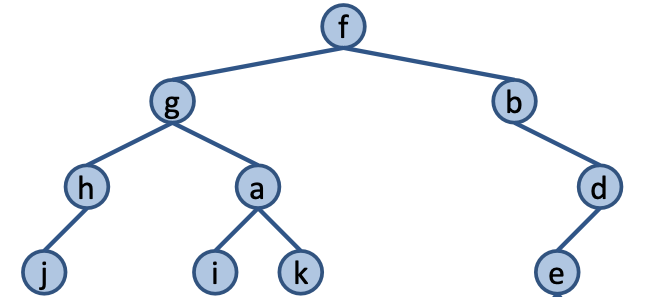
\includegraphics[width=\textwidth]{assets/IVPR.png}
  \end{minipage}
\hfill
\begin{minipage}{0.6\textwidth}
    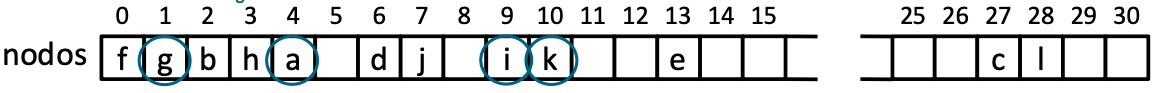
\includegraphics[width=\textwidth]{assets/IVPR2.png}
    Encontramos el vector que contiene los elementos de cada nodo, asi vemos que en la posición 4 (hijo derecho de g) encontramos el elemento `a'.\\
    Ejemplo: \texttt{hder(g)} = \texttt{hder(1)} = \(2*1+2\) = 4.
\end{minipage}
\caption{Ejemplo de la representación con un vector de posiciones relativas}
\end{figure}

Esta implementación tiene una parte mala y es que encontramos un caso muy desfavorable, esto es debido a que el tamaño del vector depende de la altura del árbol, por tanto, si encontramos la ausencia de nodo en un nivel \(n \leq h\) provocará \(2^{h-n+1}-1\) posiciones libres en el vector.

Veámoslo con un ejemplo:
\begin{figure}[h]
  \begin{minipage}{0.39\textwidth}
    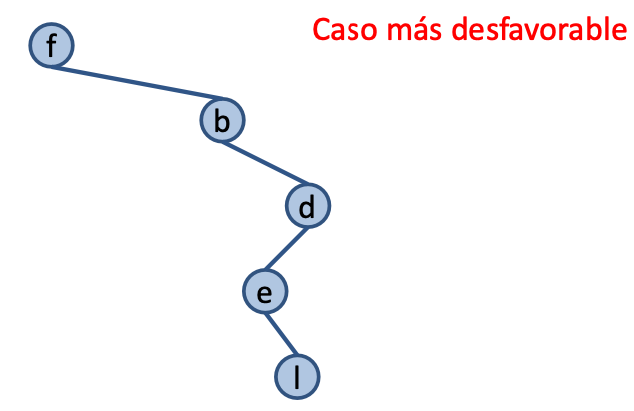
\includegraphics[width=\textwidth]{assets/IVPR3.png}
  \end{minipage}
  \hfill
  \begin{minipage}{0.6\textwidth}
    \includegraphics*[width=\textwidth]{assets/IVPR4.png}
    Si queremos que el nodo con elemento \(l\)(posición 28) tenga tanto hijo izquierdo como derecho, estos quedarán en las posiciones del vector \(2*28+1 = 57\) y \(2*28+2 = 58\) del vector, es decir, duplicamos el tamaño del vector solamente para insertar 2 nuevos nodos, un gasto de memoria excesivo.
  \end{minipage}
\end{figure}
\newpage
Por otro lado, tenemos un caso muy favorable y sucede cuando tenemos el árbol casi completo, es decir, no hay ausencia de nodos por nivel (todos los niveles tienen todos los nodos que les corresponde), lo denominamos como \textbf{árbol completo}.

\begin{figure}[h]
  \begin{minipage}{0.39\textwidth}
    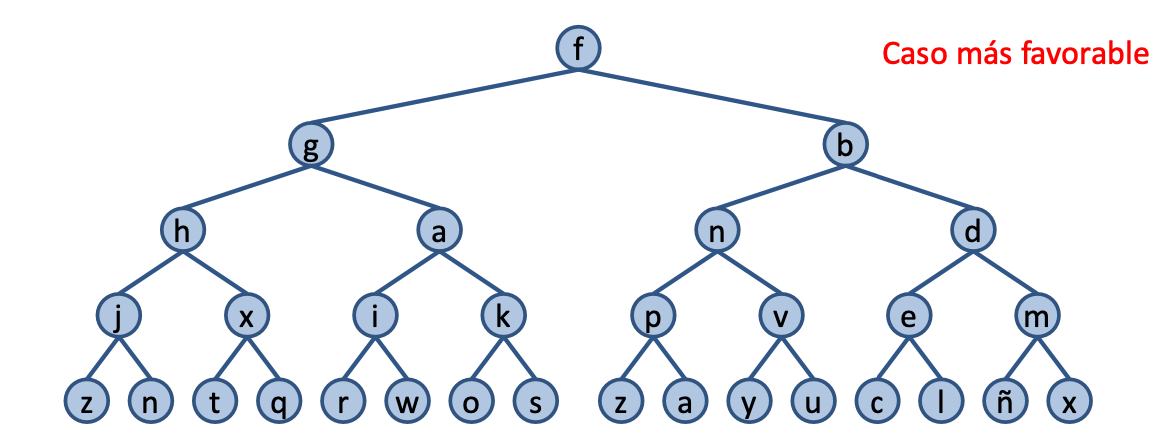
\includegraphics[width=\textwidth]{assets/IVPR5.png}
  \end{minipage}
  \hfill
  \begin{minipage}{0.6\textwidth}
    \includegraphics*[width=\textwidth]{assets/IVPR6.png}
    En esta implementación la eficiencia espacial será mejor cuanto más lleno esté el árbol, es decir, cuanto menos posiciones falten por ser rellenadas en el vector.
  \end{minipage}
\end{figure}

Finalmente, hacemos uso del concepto de \textbf{elemento nulo} \texttt{T ELTO\_NULO}, no es un elemento o contenido del nodo, si no que al igual que NODO\_NULO, indica la no existencia de elemento en el vector, es decir, una \textbf{flag} que nos indica las posiciones libres del vector (\textit{Figura 2.3:Vector nodos con el uso de elemento nulo}).
\begin{figure}[h]
  \begin{center}
    \includegraphics*[width=\textwidth]{assets/IVPR7.png}
  \end{center}
  \caption{Vector nodos con el uso de elemento nulo}
\end{figure}